\documentclass{article}
\usepackage[utf8]{inputenc}
\usepackage{indentfirst}
\setlength{\parindent}{1em}
\usepackage{graphicx} 
\usepackage{geometry}
\usepackage{amsmath}

\geometry{a4paper,scale=0.8}


\title{Artificial Immune Network Model}
\author{Zhong Wenfeng \quad 21721234}
\date{April 2018}

\begin{document}

\maketitle

\section{the Immune System}
To begin, we shall sketch a few aspects of the human adaptive immune system. A number of concepts and technical terms will be introduced to make the reader familiar with the terminology. Master details about the immune network theory and the clonal selection principle will be given in dedicated sections. An interested reader shall refer to Janeway Jr. & Travers for an introductory text in immunology and de Castro & Von Zuben for immunology under the AI perspective. The immune system is a complex of cells, molecules and organs with the primary role of limiting damage to the host organism by pathogens (called antigens, Ag), which elicit an immune response. One type of response is the secretion of antibody molecules by B cells (or Blymphocytes). Antibodies (Ab) are Y-shaped receptor molecules bound on the surface of a B cell with the primary role of recognizing and binding, through a complementary match, with an antigen. The Ab recognizes a portion of the Ag called its epitope. An idiotype is defined as the set of epitopes displayed by the variable regions of a set of Ab, and an idiotope is each single idiotypic epitope. While each B cell is known to have a single type of Ab, thus being called monospecific, an Ag typically has several different types of epitopes, and can be recognized by several different antibodies. The antibody portion responsible for matching (recognizing) an antigen is called paratope, also known as V-region, for variable region. It is variable because it can alter its shape to achieve a better match (complementarily) with a given antigen. The strength and specificity of the Ag-Ab interaction is measured by the affinity of their match. Figure 1 illustrates an Ag with its many epitopes and an Ab with its paratope and idiotope. In order to be protective, the immune system must learn to distinguish between our own (self) cells and malefic external (nonself) invaders. This process is called self/nonself discrimination: those cells recognized as self do not promote an immune response, while the unrecognized ones provoke a reaction.
\begin{center} 
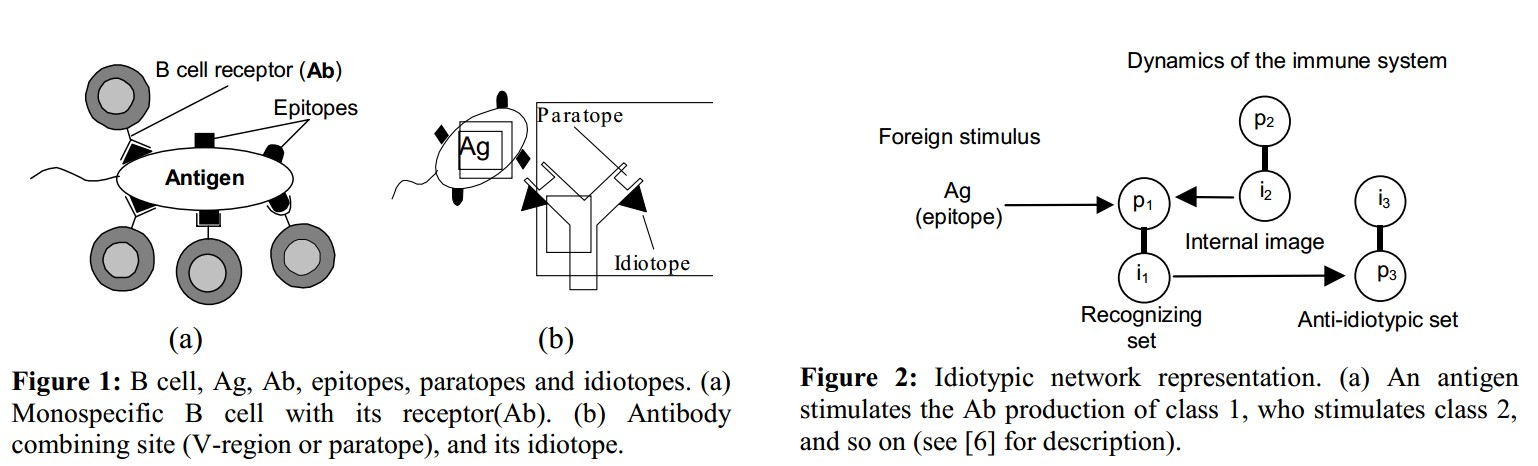
\includegraphics[width = .8\textwidth]{images/Figure_1&2.jpg}
\end{center} 


\section{Immune Network Theory}
The immune network theory, as originally proposed by Jerne , hypothesized a novel viewpoint of lymphocyte activities, natural Ab production, pre-immune repertoire selection, tolerance, self/nonself discrimination, memory and the evolution of the immune system. The immune system was formally defined as an enormous and complex network of paratopes, that recognize sets of idiotopes, and of idiotopes, that are recognized by sets of paratopes. The relevant events in the immune system are not only the molecules, but also their interactions. The immune cells can respond either positively or negatively to the recognition signal. A positive response would result in
cell proliferation, activation and antibody secretion, while a negative response would lead to tolerance and suppression. Figure 2 depicts the immune network idea.
In the model proposed by Varela & Coutinho , we can stress three characteristics of the immune networks:1) its structure, that describes the types of interaction among the network components, represented by matrices of connectivity; 2) its dynamics, that accounts for the variation in time of the concentrations and affinities of its cells; and 3) its metadynamics, a property addressed to the continuous production of novel antibodies and death of non-stimulated or self-reactive cells. The central characteristic of the immune network theory is the definition of the individual’s molecular identity (internal images), which emerges from a network organization followed by the learning of the molecular composition of the environment where the system develops.The network approach is particularly interesting for the development of computer tools because it potentially provides a precise account of emergent properties such as learning and memory, self-tolerance, size control and diversity of cell populations. In general terms, the structure of most network models can be represented as

RPV=(influx of new cells) − (death of unstimulated cells) + (reproduction of stimulated cells)

where RPV is the rate of population variation, and the last term includes Ab-Ab recognition and Ag-Ab stimulation.




\section{Typical Artificial Immune Networks}
In this section, a few representative artificial immune network models are introduced. We will discuss these models’ theory, structures, and learning algorithms in details.

\begin{center}
    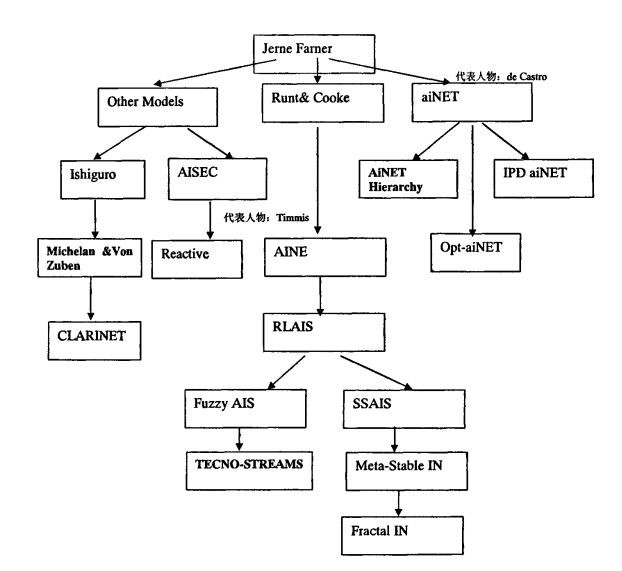
\includegraphics[width=.8\textwidth]{images/Figure_3.jpg}\\
    \captionof{Figure 3. Relationship of AIN}
\end{center}


\begin{center}
    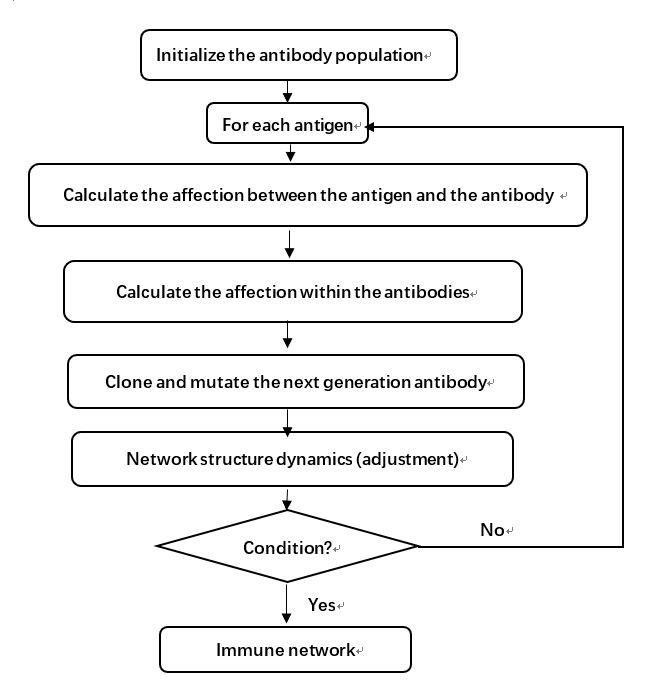
\includegraphics[width=.8\textwidth]{images/Figure_4.jpg}\\
    \captionof{Figure 4. Basic Framework of AIN}
\end{center}
\subsection{Resource Limited Artificial Immune System}
The Resource Limited Artificial Immune System (RLAIS) is built upon the work of the basic AIS . As we know, the AIS consist of a set of B cells, links among themselves via
their stimulation levels, and cloning and mutation operations performed on these B cells. The AIS can cluster together similar patterns in the training data presented. This network of B cells represents clusters with the affinity links . However several critical parameters should be manually set for efficient initialization: number of iterations, the Network Affinity Threshold (NAT), and mutation rate , which are explained as follows .
\begin{itemize}
    \item {(1) The number of iterations that the training data are presented to a learning system is not straightforward to choose. There is no direct correlation between the number of iterations and linkage value. Nevertheless, some experiences-based observations are clear: a). the more times the training set is presented to the artificial immune network, the longer it takes for the network to converge. In fact, there is an exponential growth in the network size, regardless of the training set, mutation rate, and NAT. b). We do not have a definite border line between presenting the training data in an insufficient or excessive number of times. Too many presentations of the training data may lead to a large network that is difficult interpret. The appropriate selection of this initialization parameter is clearly vital in the successful training of the AIS Figure 5 of tracks the evolution procedure of the RLAIS with the Iris data set as the training samples. Figure 5 (a) shows the resulting network after two iterations. It clearly demonstrates one separate cluster from the main cluster. Figure 5 (b) illustrates the network after five iterations, from which it is nearly impossible to observe any network structure.
}
    \item {(2) The NAT is defined in (1), which is calculated by parsing the training data and finding the average Euclidean distance between each item. In (1), li represents the affinity associated with the ith link in the network, nl is the number of links present, and A is a constant value, where 0≤A≤1.
    \[{NAT}=A \frac{\{\sum_{i=0}^{nl}{aff}(l_i)\}}{nl}  \]
    If the affinity between two B cells is less than the NAT, a link is created between them. As a matter of fact, the NAT directly influences the network linkage, and it should be
chosen as a small value, e.g., 0.1, which can decrease the potential connectivity of the AIS, and, thus, separate out the training data more efficiently than if it has larger values.
    \begin{center}
    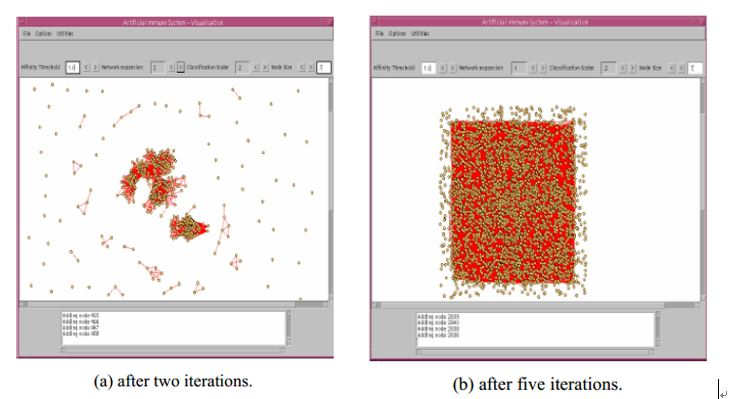
\includegraphics[width=.8\textwidth]{images/Figure_5.jpg}\\
    \captionof{Figure 5. RLAIS-based clustering of Iris data set}
    \end{center}
    }
    \item {(3)Since the mutation rate creates a diverse representation of the training data, it can reduce the connectivity in the AIS. If the mutation rate is higher, it will produce a network with fewer B cells. Figure 6 shows the growth of the network linkage over training time with a mutation rate of 10\% on the Iris data set
    \begin{center}
    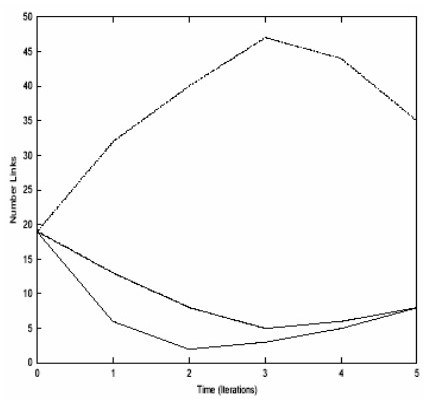
\includegraphics[width=.6\textwidth]{images/Figure_6.jpg}\\
    \captionof{Figure 6. Linkage growth with mutation rate of 10\% on Iris data set}
    \end{center}
    The main difference between an AIS and a RLAIS is the removal of the number of times the training data set is  presented to the network . The RLAIS does not require setting the number of training cycles beforehand, but can still offer a more effective population control strategy. These improvements are due to the deployment of the Artificial Recognition Ball (ARB). The ARB is a representation of a certain number of identical B cells, because individual B cells are no longer explicitly represented in the RLAIS. The RLAIS has a group of ARBs as well as links among them. All the ARBs compete for representing the B cells within the RLAIS on the basis of their stimulation levels. The higher the ARB stimulation level, the more B cells it can represent. Once an ARB does not represent any B cells, it is expunged from the network. Indeed, the goal of the mutation mechanism is to create new ARBs that can better fit the training data. As new ARBs are created, some of them are satisfactory matching of the training data, while others are not. The latter are less stimulated by the training data and network, and will be ultimately removed from the RLAIS. The ‘base’ size of the network is obtained after a number of training iterations. Thus, over-training is not a serious problem in the RLAIS. The explosion in population growth can be eliminated by the above new population control scheme. Clearly, compared with the AIS population growth, no exponential growth exists in the RLAIS. Additionally, instead of recalculating the NAT at the end of each training epoch in the AIS, we keep it constant throughout the whole learning process in the RLAIS. The RLAIS can be also used as a solid basis for continuous learning: previously unseen input data is presented to the 
RLAIS to allow new patterns to be learnt without adversely affecting those patterns already learnt. Unfortunately, there are a few unsolved problems in designing our RLAIS. For example, choosing the number of B cells that the RLAIS should allocate is an important factor. If there are too many resources selected, the network will become too large and unrepresentative, while too few resources can result in some un-captured patterns. Reference proposes a new Self-Stabilizing Artificial Immune System (SSAIS) to deal with this drawback. The SSAIS differs from the RLAIS in that there is no fixed quantity of resources to be centrally distributed among the ARBs. The concept of resources is still used, but in an altered way. In the SSAIS, the resources are handled locally by each ARB. The ARB can increase its own resource allocation, when it registers the highest stimulation for an incoming data sample .

    }
\end{itemize}
\subsection{aiNet}
The aiNet is an emerging kind of the AIS inspired by the immune network theory firstly proposed by Jerne in 1974. It is developed based on the ideas and concepts of three theories: the immuned network theory, the clonal selection principle, and affinity maturation principle . The main role of this artificial immune network is to perform data
compression by following the clonal selection as well as affinity maturation principles. The immune network theory hypothesizes the activities of the immune cells, emergence of memory, and discrimination between our own cells (known as self) and external invaders (known as non-self). The aiNet model consists of a group of cells, namely antibodies, interconnected by links with associated connection strengths. The aiNet antibodies represent the network internal images of the pathogens (input patterns), to which they are exposed. The connections among these antibodies determine their interrelations with providing a degree of similarity among themselves in the given metric space. The closer the antibodies, the more similar they are. This approach results in an antibody network that can recognize the antigens (input data set) with an adjustable generality. The aiNet learning procedure can be divided in two principal steps . The first one corresponds to the clonal selection principle and affinity maturation interactions, where the antibodies (Ab) suffer from the cloning and mutation in order
to recognize the antigens (Ag). This stage is actually similar to the CLONal selection ALGorithm (CLONALG) originally proposed by de Castro and von Zuben. The raw training data set is explored and compressed by the aiNet leading to an antibody network that extracts the most relevant information from the data for the clustering purposes. The second step of the aiNet includes the immune network interactions and introduction of diversity. The Minimal Spanning Tree (MST) is built on the antibody network, and its inconsistent edges are identified and removed, which can transform the network (data) separation into clusters.
In general, the aiNet is developed to answer the following important questions: is there a great amount of redundancy within the training data set, and, if there is, how can we reduce it? Are there any subgroups intrinsic to the data? How many groups are there in the input data set? What is the structure of the spatial distribution of these data? How can we generate decision rules to classify novel samples? However, the main drawbacks of the aiNet, as pointed out in , are the large number of application dependent parameters and processing overhead of each iteration. The aiNet can be considered as an evolutionary artificial immune network, because the evolution strategies based on
the genetic variation and selection within a population of individuals are used to control the network dynamics and plasticity. Reference proposes that the aiNet is capable of
detecting the optimal solutions. Combined with the constant modulus criterion, it has been employed for the optimal blind IIR equalization. Furthermore, the aiNet is also a connectionist system, in which a matrix of connection strengths is defined to measure the affinities among the network cells. The learning algorithm targets at building a memory set that can recognize and represent the structural organization of the training data. Especially, the suppression threshold controls the specificity level of the cells, clustering accuracy, as well as network plasticity.

\subsection{iNet}
The iNet is a general framework for simulating the natural immune networks and further describing how to develop the AIS . It utilizes the essential principles of the AIS, such as autonomous policy negotiation and system reconfiguration facility, for communication. The iNet serves as an information infrastructure, and can be applied to explore related mechanisms. Additionally, it helps to investigate a family of applications based on the artificial immune networks. As we know, application frameworks and patterns can enhance the reuse techniques, reduce development cost, and improve the quality of applications. The reusable components within the iNet are
designed with several software patterns. Therefore, the iNet can explicitly show the developers its design intents and extension points, with which they can effectively tailor their own applications. More precisely, it is designed to allow the proper customization of various strategies to construct the artificial immune networks, e.g., network topology and network dynamics control. The iNet contains four main packages:GUI visualization, graph management, immuno-component management, and persistence & exchange, as illustrated in Figure 7.
    \begin{center}
    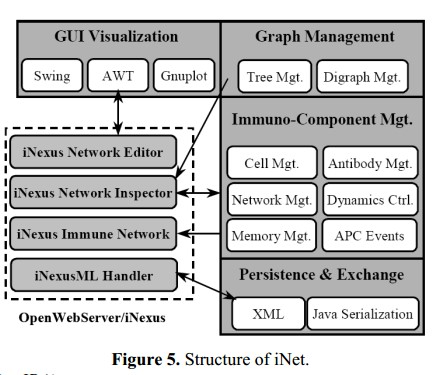
\includegraphics[width=.6\textwidth]{images/Figure_7.jpg}\\
    \captionof{Figure 7. Structure of iNet}
    \end{center}
\section{Applications of Artificial Immune Network}
During the past decade, the artificial immune networks have been successfully applied to a large variety of engineering areas, such as data mining , time series prediction, pattern recognition , optimization, fault detection , computer security , and process control. In this section, a few examples of these applications are demonstrated and discussed. We will also present our work on the clustering applications of the AIS. It illustrates that our AIS-based clustering algorithm is better than the commonly used clustering method, K-means.
\subsection{Multimodal function optimization}
Optimization is a popular application area for the artificial immune networks. Reference presents a modified version of the artificial immune network model specially designed to cope with multimodal optimization problems. It is theoretically compared with the clonal selection algorithm concerning their evolution strategies. A new artificial immune optimization method, named CLONALG to perform pattern recognition and engineering optimization. The authors empirically demonstrate that the CLONALG is capable of learning the input patterns by selecting, reproducing, and mutating a set of ‘artificial immune cells’. 
The aforementioned aiNet combining the CLONALG with the artificial immune network theory has been successfully applied in several data compression and clustering applications including non-linear separable and high-dimensional problems. The same rationales that lead to the CLONALG are the motivations for the optimization version of the aiNet, namely opt-aiNet. Firstly, data clustering can be considered as an optimization problem, where each cluster corresponds to the fitness peak of a subgroup of individuals within the whole population. Secondly, the aiNet is an extension of the CLONALG with additional steps involving the stimulation/suppression interaction of the network cells with each other. The advantage of evaluating the degree of similarity among the cells is that it is possible to maintain a dynamic control of the number of network cells, which allows the ultimate finding of more parsimonious solutions.
The opt-aiNet has been deployed to optimize several uniand bi-dimensional functions to assess its optimization performance. The results are also compared with those obtained by the CLONALG. In , three nonlinear functions are explored: multi, roots, and Schaffer’s. Figure 8 illustrates the performances of both the CLONALG and opt-aiNet, when employed to the same multimodal function optimization problem. Apparently, the opt-aiNet locates 61 peaks, while the CLONALG locates only 18. Moreover, the opt-aiNet positions one single individual in each peak, which can overcome the harmful ‘waste of resources’ shortcoming of the CLONALG. 
\begin{center}
    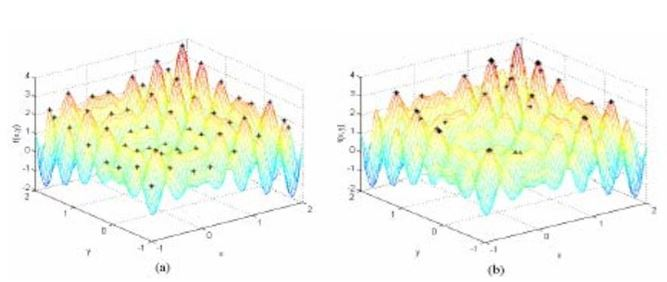
\includegraphics[width=.6\textwidth]{images/Figure_8.jpg}\\
    \captionof{Figure 8. Multimodal function optimization (a) using opt-aiNet (b) using CLONALG}
    \end{center}
\subsection{Pattern recognition}
   Reference proposes a new artificial immune network with diversity based on the ideas borrowed from the living body immune system, whose dynamics are examined via
computer simulations on alphabet pattern recognition. The memory patterns in this system are classified into three unique types, as given in Figure 9 . Pattern recognition is performed using the artificial immune network with these memory patterns of such three types. More precisely, Type 1: in a certain fixed preprocessing period, the input pattern becomes the memory pattern. Here, the memory pattern does not update,and, therefore, is retained in the present state. Type 2: when the input pattern has been recognized to be a memory pattern belonging to Type 1, the corresponding memory pattern in Type 2 is updated with the memory pattern and input pattern of the recognized Type 1. Type 3: the memory pattern of this type has the similarity between the updated memory pattern in Type 2 and original memory pattern (memory pattern in Type 1) of M% or above. Moreover, the memory pattern recognized and memorized as an unknown pattern also belongs to Type 3.Note that, in Type 3, the memory pattern, which is not continuously updated for L times, will be deleted . Reference investigates the application of the above artificial immune network in the pattern recognition system
for alphabets. The rate of correct recognition, rate of incorrect recognition, and rate of rejection are employed to evaluate the system performance. Furthermore, the proposed artificial immune network is compared with the binary immune network in order to access its noise tolerance and recognition capabilities, when presented to the binary noise. Simulation results show that with the network diversity, it can acquire stronger noise immunity than the binary immune network for binary input patterns.
    \begin{center}
    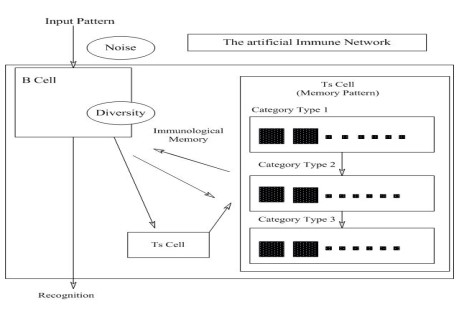
\includegraphics[width=.6\textwidth]{images/Figure_9.jpg}\\
    \captionof{Figure 9 Pattern recognition using artificial immune network}
    \end{center}

\end{document}
